\section{Background on Rational Proofs}

\begin{frame}{Overview of Rational Proofs [AM12]}
\begin{itemize}[<+- | alert@+>]
	\item A variant of interactive proofs where the verifier pays the prover at the end;
	\item \textbf{Soundness:}
	\begin{itemize}
		\item ``A cheating worker gains less than an honest one''
	\end{itemize}
%	\item Other desiderata:
%	\begin{itemize}
%		\item Reward should be higher than cost (\textit{individually rational})
%		\item Ensuring ``significant'' losses for cheaters;
%		\item Ensuring ``compact'' budget for delegators.
%	\end{itemize}
\end{itemize}
% Recall interactive proofs
% Recall our goal
\end{frame}


\begin{frame}{Rational Proofs: Definition [AM12]}
		\begin{framed}
			Let $f$ be a function and $(P,V)$ be a pair of algorithms. $(P,V)$ is a rational proof for $f$ if both:
			\onslide<+->
			\begin{enumerate}[<+- | alert@+>]
				\item \emph{("The honest prover always replies correctly")} 
				$$ \forall x\  \Pr[output(P,V)(x) = f(x) ] = 1$$
				\item \emph{("Any other prover will earn less than the honest one")}
				$$ \forall \disP \ \forall x \  \expRewProtHon \geq \expRewProtDis + \delta_{\disP}(x)  $$
				for some reward function $\rew$ and gap $\delta_{\disP}(x) \geq 0$
			\end{enumerate}
		\end{framed}
		
		\pause
		\vspace{0.5cm}
		\center{\large{\textbf{What does $\rew$ look like?}}}
\end{frame}

\begin{frame}{One Approach to Reward Functions: Scoring Rules [AM12]}
	% What  to put in here??

\begin{itemize}[<+- | alert@+>]
	\item Consider a (probabilistic) forecasting $\textbf{p} = (p_1,...,p_m)$ \\
	(e.g. $\textbf{p} = (\text{\emph{Rain}} : .6, \text{\emph{Sun}} : .3, \text{\emph{Snow}} : .1)$ )
	\item A \emph{scoring rule} $S$ rewards an expert 
	$$ S(\textbf{p}, \omega) $$ 
	for forecasting $\textbf{p}$ on realized outcome $\omega$.
	% In other words, S is a function that given a forecast and an outcome provides a reward.
	% In the weather case we can look the observed outcome can be "the weather you observe tomorrow".
	% This is the main idea behind scoring rule, but we need one more property to incentive 
	\item \emph{Proper} scoring rules: 
	\begin{itemize}
		\item incentivize experts to provide correct forecasting;
		\item $\expectation_{\omega}[S(\textbf{p}, \omega)]$ is max \emph{iff} the forecasting $\textbf{p}$ is \emph{the real} distribution.
	\end{itemize}
	
\end{itemize}

\onslide<+->
\center{\large{\textbf{What do proper scoring rules look like?}}}

% Intuition on scoring rule
\end{frame}

\begin{frame}{Example: Scoring Rules for a Binary Domain}
	% In this slide we look at a specific scoring rule
	\begin{itemize}[<+- | alert@+>]
		\item Consider simplified weather forecasting problem: only two outcomes are \emph{Sunny} (S) and \emph{Cloudy} (C).
		\item ``Expert'' declares alleged $\tilde{p}_S$ and we observe the weather.
		\item For each outcome (i.e. Sunny and Cloudy):
		\begin{itemize}
			\item $BSR(\tilde{p}_S, S) = 2\tilde{p}_S(2-\tilde{p}_S)$
			\item $BSR(\tilde{p}_S, C) = 2(1-\tilde{p}_S^2)$
		\end{itemize}
		\item Maximized in expectation  when $p_S = \tilde{p}_S$
		\item $0 \leq BSR(\cdot, \cdot) \leq 2$
		%\item Notice that $0 \leq BSR(\cdot, \cdot) \leq 2$ but can be scaled appropriately (e.g. by $\poly(n)$).
		
	\end{itemize}
	
	%\onslide<4->\hline
	\bigskip
	\bigskip
	
	\onslide<4->\small{BSR: Brier's Scoring Rule [Brier50]}
	
\end{frame}

\begin{frame}{A Simple Rational Proof for Threshold Gates [AM13]} 
\begin{block}{Threshold Circuit}
	Each gate outputs 1 iff input has at least $k$ bits equal to 1.
\end{block}
\pause
\noindent
\begin{columns}
	\column{0.55\textwidth}
	Let:
	\begin{itemize}[<+- | alert@+>]
		\item input $x \in \binstring^n$
		\item $i$ be the  \# of bits of $x$ equal to 1.
		\item \emph{Example:} on input $x=10110$ $i=3$. 
	\end{itemize}
	\pause
	
	\begin{block}{\textbf{The protocol}  (for one gate):}
		
		\begin{itemize}[<+- | alert@+>]
			\item $P$ to $V$: "There are $\tilde{i}$ bits equal to 1 in x"
			\item \textbf{Output:} $V$'s output is 1 iff $\tilde{i} \geq k$
			\item \textbf{Computing reward:}
			\begin{itemize}
				\item $V$ samples a bit $b$ of the input
				\item $V$ pays $BSR(\frac{\tilde{i}}{n}, b)$
			\end{itemize}
		\end{itemize}
	\end{block}
	\onslide<1->
	\column{0.45\textwidth}
	\begin{figure}
		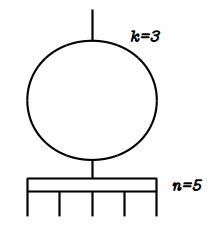
\includegraphics[scale=0.8]{pics/threshold-circ.png}
		
	\end{figure}
\end{columns}
\end{frame}


\begin{frame}{Rational Proofs - Recap}
	\begin{itemize}[<+- | alert@+>]
		\item Variant of interactive proof with incentive-based soundness;
		\item One way to obtain them: scoring rules;
		\item Rational proofs for threshold circuits.
	\end{itemize}
\end{frame}